\chapter{Chapter 1}
We, the group, wanted to work with an unstable system for this bachelor project in control engineering. The choice fell on a form of inverted pendulum. It is a setup called Cubli, wich is a cube that can jump up and balance on one of its sides or on one of its corners.

The Cubli is designed as a simple setup to let control engineers work with an inverted pendulum. A working cubli also can be a fun thing to show the general public to explain what control engineering is about.  \cite{MGajamohan}

\begin{figure}[H] 
	\centering 
	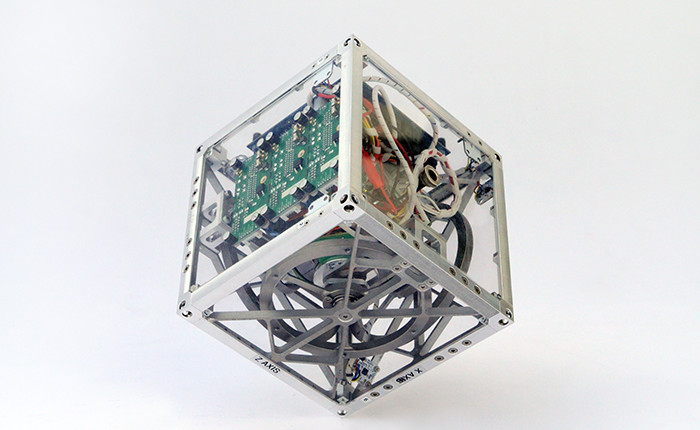
\includegraphics[scale=1.5]{figures/CubliCorner-700x430}
	\caption{A Cubli balancing on one of its corners\cite{RAndrea}}
	\label{CubliCorner}
\end{figure} 

The Cubli balances with the help of reaction wheels that spin up or down. Jumping up from a resting position is done by braking one or more of the reaction wheels, wich overcomes the friction keeping the cubli still. 

Applications for this Cube, that moves without any external tools, might seem limited when you only have one cube. If you take a group of cubes, they could move together to traverse obstacles one cube alone could not. \cite{JRomanishin}



%At AAU we have a one-dimensional setup, based on the Cubli idea. It consists of a metalframe with one flywheel. In this case the inverted pendulum setup is not controlled by a motor that moves the pendulum, but by a flywheel attached to the square frame. The idea is to balance the frame on one corner with the help of the flywheel by accelerating the wheel up and down.


